\subsection{Events}

\begin{table}[h]
	\centering
	\resizebox{\columnwidth}{!}{
	\begin{tabular}{||c | c | c | c||} 
		\hline
		\textbf{Event} & \textbf{System Response} & \textbf{Source} & \textbf{Type}\\
		\hline\hline
Luminosity detector OFF & Power the lamp & Environment & Asynchronous\\\hline
LED failure detector ON & Notify remote system & Local system & Asynchronous\\\hline
Motion detected & Turn on the lamp & User & Asynchronous\\\hline
Requested to turn on the lamp & Turn on the lamp & Local system & Asynchronous\\\hline
Camera sample & Image processing & Timer & Synchronous\\\hline
Update system information & Send data to remote system & Local system & Asynchronous\\
		\hline
	\end{tabular}
	}		
	
	\caption{Base station events.}
	\label{table:data}
\end{table}


\subsection{Use Cases}

\begin{figure}[ht]
	\centering
	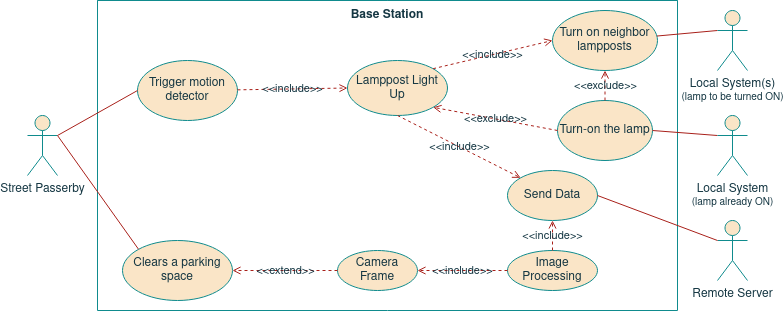
\includegraphics[width=.85\textwidth]{/05base_station/BS_UseCase}
	\caption{Base station use cases.}
	\label{fig:bs_use_cases}
\end{figure}

\subsection{State Chart}

\begin{figure}[ht]
	\centering
	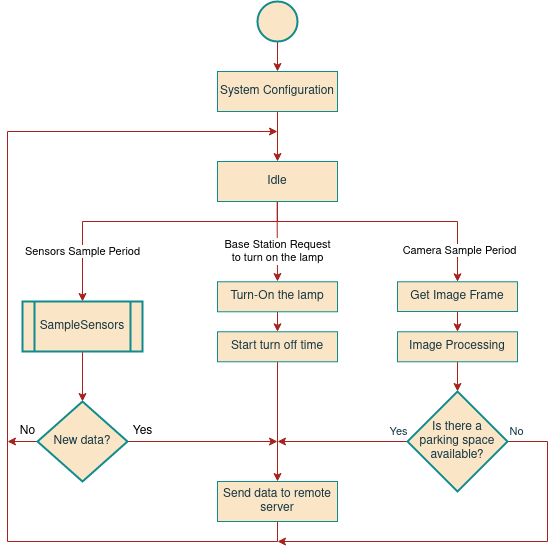
\includegraphics[width=.85\textwidth]{/05base_station/BS_StateChart}
	\caption{Base station state chart.}
	\label{fig:bs_state_chart}
\end{figure}

\begin{figure}[ht]
	\centering
	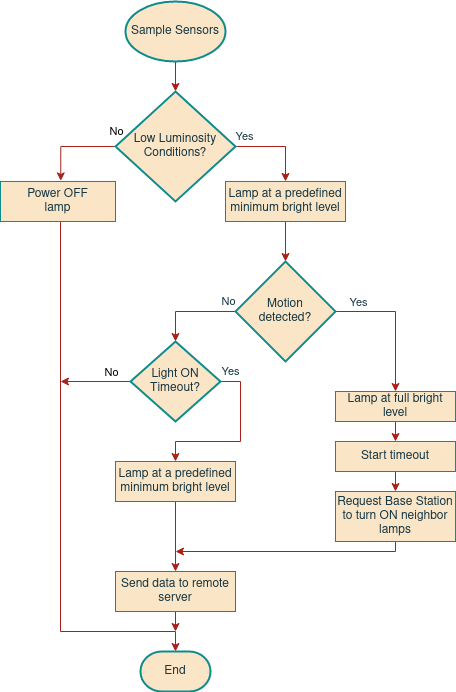
\includegraphics[width=.85\textwidth]{/05base_station/SampleSensors}
	\caption{Sampling of the sensors state chart.}
	\label{fig:sample_sensors}
\end{figure}

\subsection{Sequence Diagram}

\begin{figure}[ht]
	\centering
	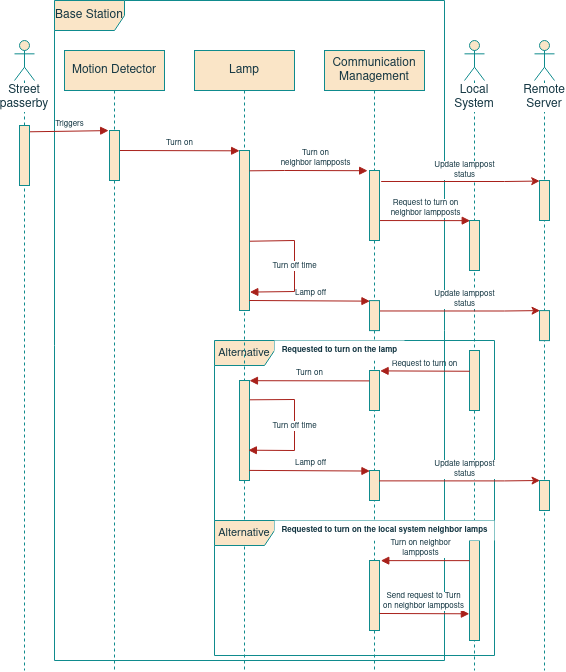
\includegraphics[width=.85\textwidth]{/05base_station/BS_SeqDiagram}
	\caption{Base station sequence diagram.}
	\label{fig:bs_seq_diagram}
\end{figure}